\documentclass[a4paper,12pt]{article}
\usepackage{pre} % преамбула и настр


\title{Стекло и метеориты}
\author{И.\,И.\,Кравченко}


\begin{document}


\renewcommand\refname{Литература}


\maketitle


Решаем задачу по физике про наложение и отражение волн из сборника Савченко~\cite{sa08}. Опубликовано впервые на \href{https://savchenkosolutions.com/ru/3.8.7}{<<Savchenko Solutions>>}.

\medskip

\def\fw{\linewidth-2\fboxsep-\fboxrule}
\noindent\fbox{%
    \parbox{\linewidth-2\fboxsep-2\fboxrule}{%
    \textbf{3.8.7.} На внешней стороне стекла иллюминатора космического корабля имеются разрушения, вызванные попаданием микрометеоритов. Подобные же разрушения видны на внутренней стороне. Объясните их появление.%
    \begin{center}
        \includesvg[width=.4\linewidth]{pic0}
    \end{center}
    %
    }%
}   


\section{Волна сжатия}

Качественное объяснение удобно провести через сферические волны. 

Итак, метеорит ударяется о внешнюю границу стекла. Линейный размер области удара пусть много меньше толщины разрушения в месте удара (основное разрушение). На расстояниях порядка толщины основного разрушения в стекле движется бегущая сферическая волна (выглядит как полусферическая в стекле действительно) с центром волнового фронта в месте удара. Это волна сжатия и посчитаем ее толщину~$\delta$ много меньше толщины основного разрушения (тонкая волна).
\begin{center}
    
\includegraphics[]{pic1.pdf}
\end{center}
В точке~$A$ был удар; $r$ есть расстояние от места удара до волны.

Продолжим рассуждения без учета каких-либо потерь энергии для тонкой сферической волны, которую в каждый данный момент по тонкой геометрии можно представить как состоящую из множества плоских волн, расходящихся в свою сторону.  

Пусть изменение давления~$\Delta P$ в нашей волне одинаково в каждый момент по всей толщине ее~$\delta$. Энергия в волне из соотношения для плоских равна:
$$
W=2\pi r^2\delta\cdot E\varepsilon^2,
$$
где $2\pi r^2\delta$~--- объем волны на расстоянии~$r$ от места удара, $E\varepsilon^2$~--- плотность энергии волны (тут $E$~--- модуль Юнга, $\varepsilon$~--- относительная деформация).

Откуда с учетом~$\Delta P=E\varepsilon$
$$
\Delta P=\sqrt{\frac{EW}{2\pi\delta}}\cdot\frac{1}{r}.
$$

С расстоянием от точки удара изменение давления в волне падает. Можем считать, что волна смогла разрушить стекло на расстоянии~$d$ (толщина основного разрушения), но не более, значит, максимальное выдерживаемое изменение давления сжатия
\begin{equation*}
\boxed{\Delta P_\text{сж.$\,$max}=\sqrt{\frac{EW}{2\pi\delta}}\cdot\frac{1}{d}.\tag{1}}
\end{equation*}

Распространяясь сферическим куполом изменение давления в волне убывает с расстоянием, и при $r>d$ до касания внутренней грани (стороны стекла) изменение давления сжатия меньше~$\Delta P_\text{сж.$\,$max}$ и стекло не разрушается.

\nocite{*}


\section{Волна растяжения}

Обозначим толщину стекла~$H$.

Пусть внутренняя грань идеально свободная. Мы знаем по задаче~$3.8.5$ (Савченко), что после касания фронта волны сжатия внутренней грани стекла возмущение в стекле будет результатом наложения этой прямой волны сжатия и такой же обратной волны, но растяжения, движущейся симметрично относительно свободной грани навстречу прямой волне. Обратная волна источается как будто из точки на расстоянии~$2H$ от реального места удара.
\begin{center}
    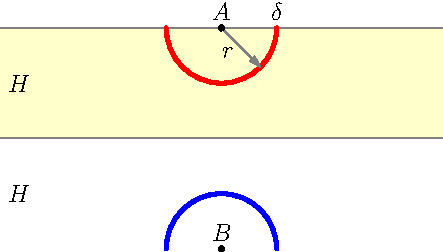
\includegraphics[]{pic2.pdf}
\end{center}
Здесь~$B$ есть мнимая точка истока обратной волны.

Не будем рассматривать тонкую область наложения прямой и обратной волн. Скажем, что через время~$\delta/(2c)$ после касания прямой внутренней грани, где $c$~--- скорость распространения волны в стекле, на расстоянии~$\delta/2$ от внутренней грани начнется появление возмущения чистого растяжения~--- это обратная волна, середина которой движется к точке удара метеорита.
\begin{center}
    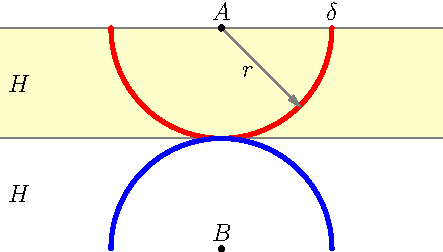
\includegraphics[]{pic3.pdf}
\end{center}
Именно с этого момента может начать разрушаться стекло через растяжение, так как прочность стекла на растяжение значительно меньше(!), чем на сжатие. Разрушение растяжением упрощенно может быть в области, где побывает только обратная волна.

В нашей модели для края разрушения растяжением (на внутренней грани стекла), толщина которого пусть~$b$, мы запишем формулу~$(1)$ применительно к обратной волне по справедливости из симметрии прямой и обратной волн:
\begin{equation*}
\boxed{\Delta P_\text{рас.$\,$max}=\sqrt{\frac{EW}{2\pi\delta}}\cdot\frac{1}{H+b}.}\tag{2}
\end{equation*}
Разделим~$(1)$ на~$(2)$ и выразим~$b$:
$$
b=\frac{\Delta P_\text{сж.$\,$max}d-\Delta P_\text{рас.$\,$max}H}{\Delta P_\text{рас.$\,$max}}.
$$

Условие существования разрушения внутри есть $b>0$, что на предыдущее накладывает
$$
\Delta P_\text{сж.$\,$max}d-\Delta P_\text{рас.$\,$max}H>0
$$
или 
$$
\boxed{d>\frac{\Delta P_\text{рас.$\,$max}}{\Delta P_\text{сж.$\,$max}}H.}
$$

При таких толщинах основного разрушения появятся разрушения на внутренней стороне.

Посмотрите, что эта модель дает близкое значение толщины откола снутри по рисунку к задаче для обычных стекол с $\dfrac{\Delta P_\text{рас.$\,$max}}{\Delta P_\text{сж.$\,$max}}\sim0{,}1$.


В книге «Физика в задачах» так же под ред. \strut О.Я. Савченко 2013 г. авторы в одной из задач предлагают тот же сюжет, но на расчет~$\dfrac{\Delta P_\text{рас.$\,$max}}{\Delta P_\text{сж.$\,$max}}$.


Посмотреть результаты экспериментов по ударам метеоритов о стекло в статье~\cite{ti76} из Новосибирска. 



\printbibliography


\end{document}